\chapter{Simulation in CUORE}
\label{ch:Simulation in CUORE}

In CUORE, simulation plays a large role in characterizing both signal and background.
As noted in \autoref{eq:sensitivity_short}, any search for \zeronubb~needs to be able to fully understand the background contribution in the region of interest.
This is certainly a non-trivial problem, however, as there are radioactive contaminants in varying levels all around the cryostat, and the data measured in CUORE is a function of all of them simultaneously.
In simulation, we can identify and study each of these particular sources in isolation or together in order to determine their effects on the data.
\section{Monte Carlo Method Overview}
The general method by which all simulation is run is called the Monte Carlo method.
The idea behind this method is a simple one: for many problems that have a computationally intractable solution, a simpler problem is to repeatedly and randomly sample possible cases to solve.

For example, calculating $\pi$ can be done via a simple Monte Carlo method by sampling random points in a unit square and dividing the number of points that are inside an inscribed circle by the total number of points.
When the sample size is large, this method works well to determine the value of $\pi$.
As noted above, in CUORE we are generally interested in determining what the distribution of timing, energy, and location of particular types of events is, and thus we apply these Monte Carlo methods to determine the effect by sampling produced particles and their interactions in the cryostat.
We also use other types of Monte Carlo, which are discussed more in \autoref{ssec:MCMC}.

An example in the case of CUORE comes from the fact that determining the energy spectrum coming from the decays in a $^{60}\textrm{Co}$ contamination on a copper frames is a difficult problem to solve analytically, but it is more straightforward to solve for the propagation and energy deposition of individual particles emitted from the copper frames.
Furthermore, these types of problems are highly parallelizable and benefit strongly from large computing clusters.

\section{Geant4 Simulation Toolkit}
The Geant4 toolkit is a software widely used in the physics community to solve these sorts of physics problems where particles pass through matter using Monte Carlo methods \cite{AGOSTINELLI2003250, 528223, ALLISON2016186}.
Using this toolkit, one can define the detector geometry and materials and then propagate particular particles with varying physics models.
As these particles move throughout these materials, their interactions and daughter particles are created and further propagated through matter.
In a detector, the energy lost by the particle and its daughters during steps inside the volume can be recorded as the energy deposited in the detector.

\section{CUORE Reconstruction in Geant4}
CUORE utilizes this software package\footnote{Version 9.6.p03} and has recreated the entire cryostat in its own software package, called \textit{qshields}, shown in \autoref{fig:CUORE_cyrostat_MC} and \autoref{fig:CUORE_crystals_MC}.
For the reconstruction, there is a balancing act in the reconstruction between the full fidelity of the recreation and the need for simplicity to reduce the load on CPU resources.
For example, there are 4 thermalizing blocks for the calibration system on the 4K stage, see \color{red}add reference to 4K thermalizer image \color{black}, but they are not included in the reconstruction of the cryostat.
The detectors and their nearest components do require as high-fidelity of a reconstruction as possible, as their particular geometry plays a significantly larger role in the simulated physics\footnote{Consider an $\alpha$ emitted from the external lead versus one from the copper frames around the detectors.
It is certainly important to each what the geometry looks like, but the $\alpha$ from the external lead will never make it to the detectors.}.
This can be seen in \autoref{fig:CUORE_crystals_MC}
In the internal and external lead shielding, particles are propagated to a minimum of 1 cm step size, as they are less likely to interact with the detectors, while the other components have a minimum step size of 0.1 cm.

\begin{figure}[htbp]
    \centering
    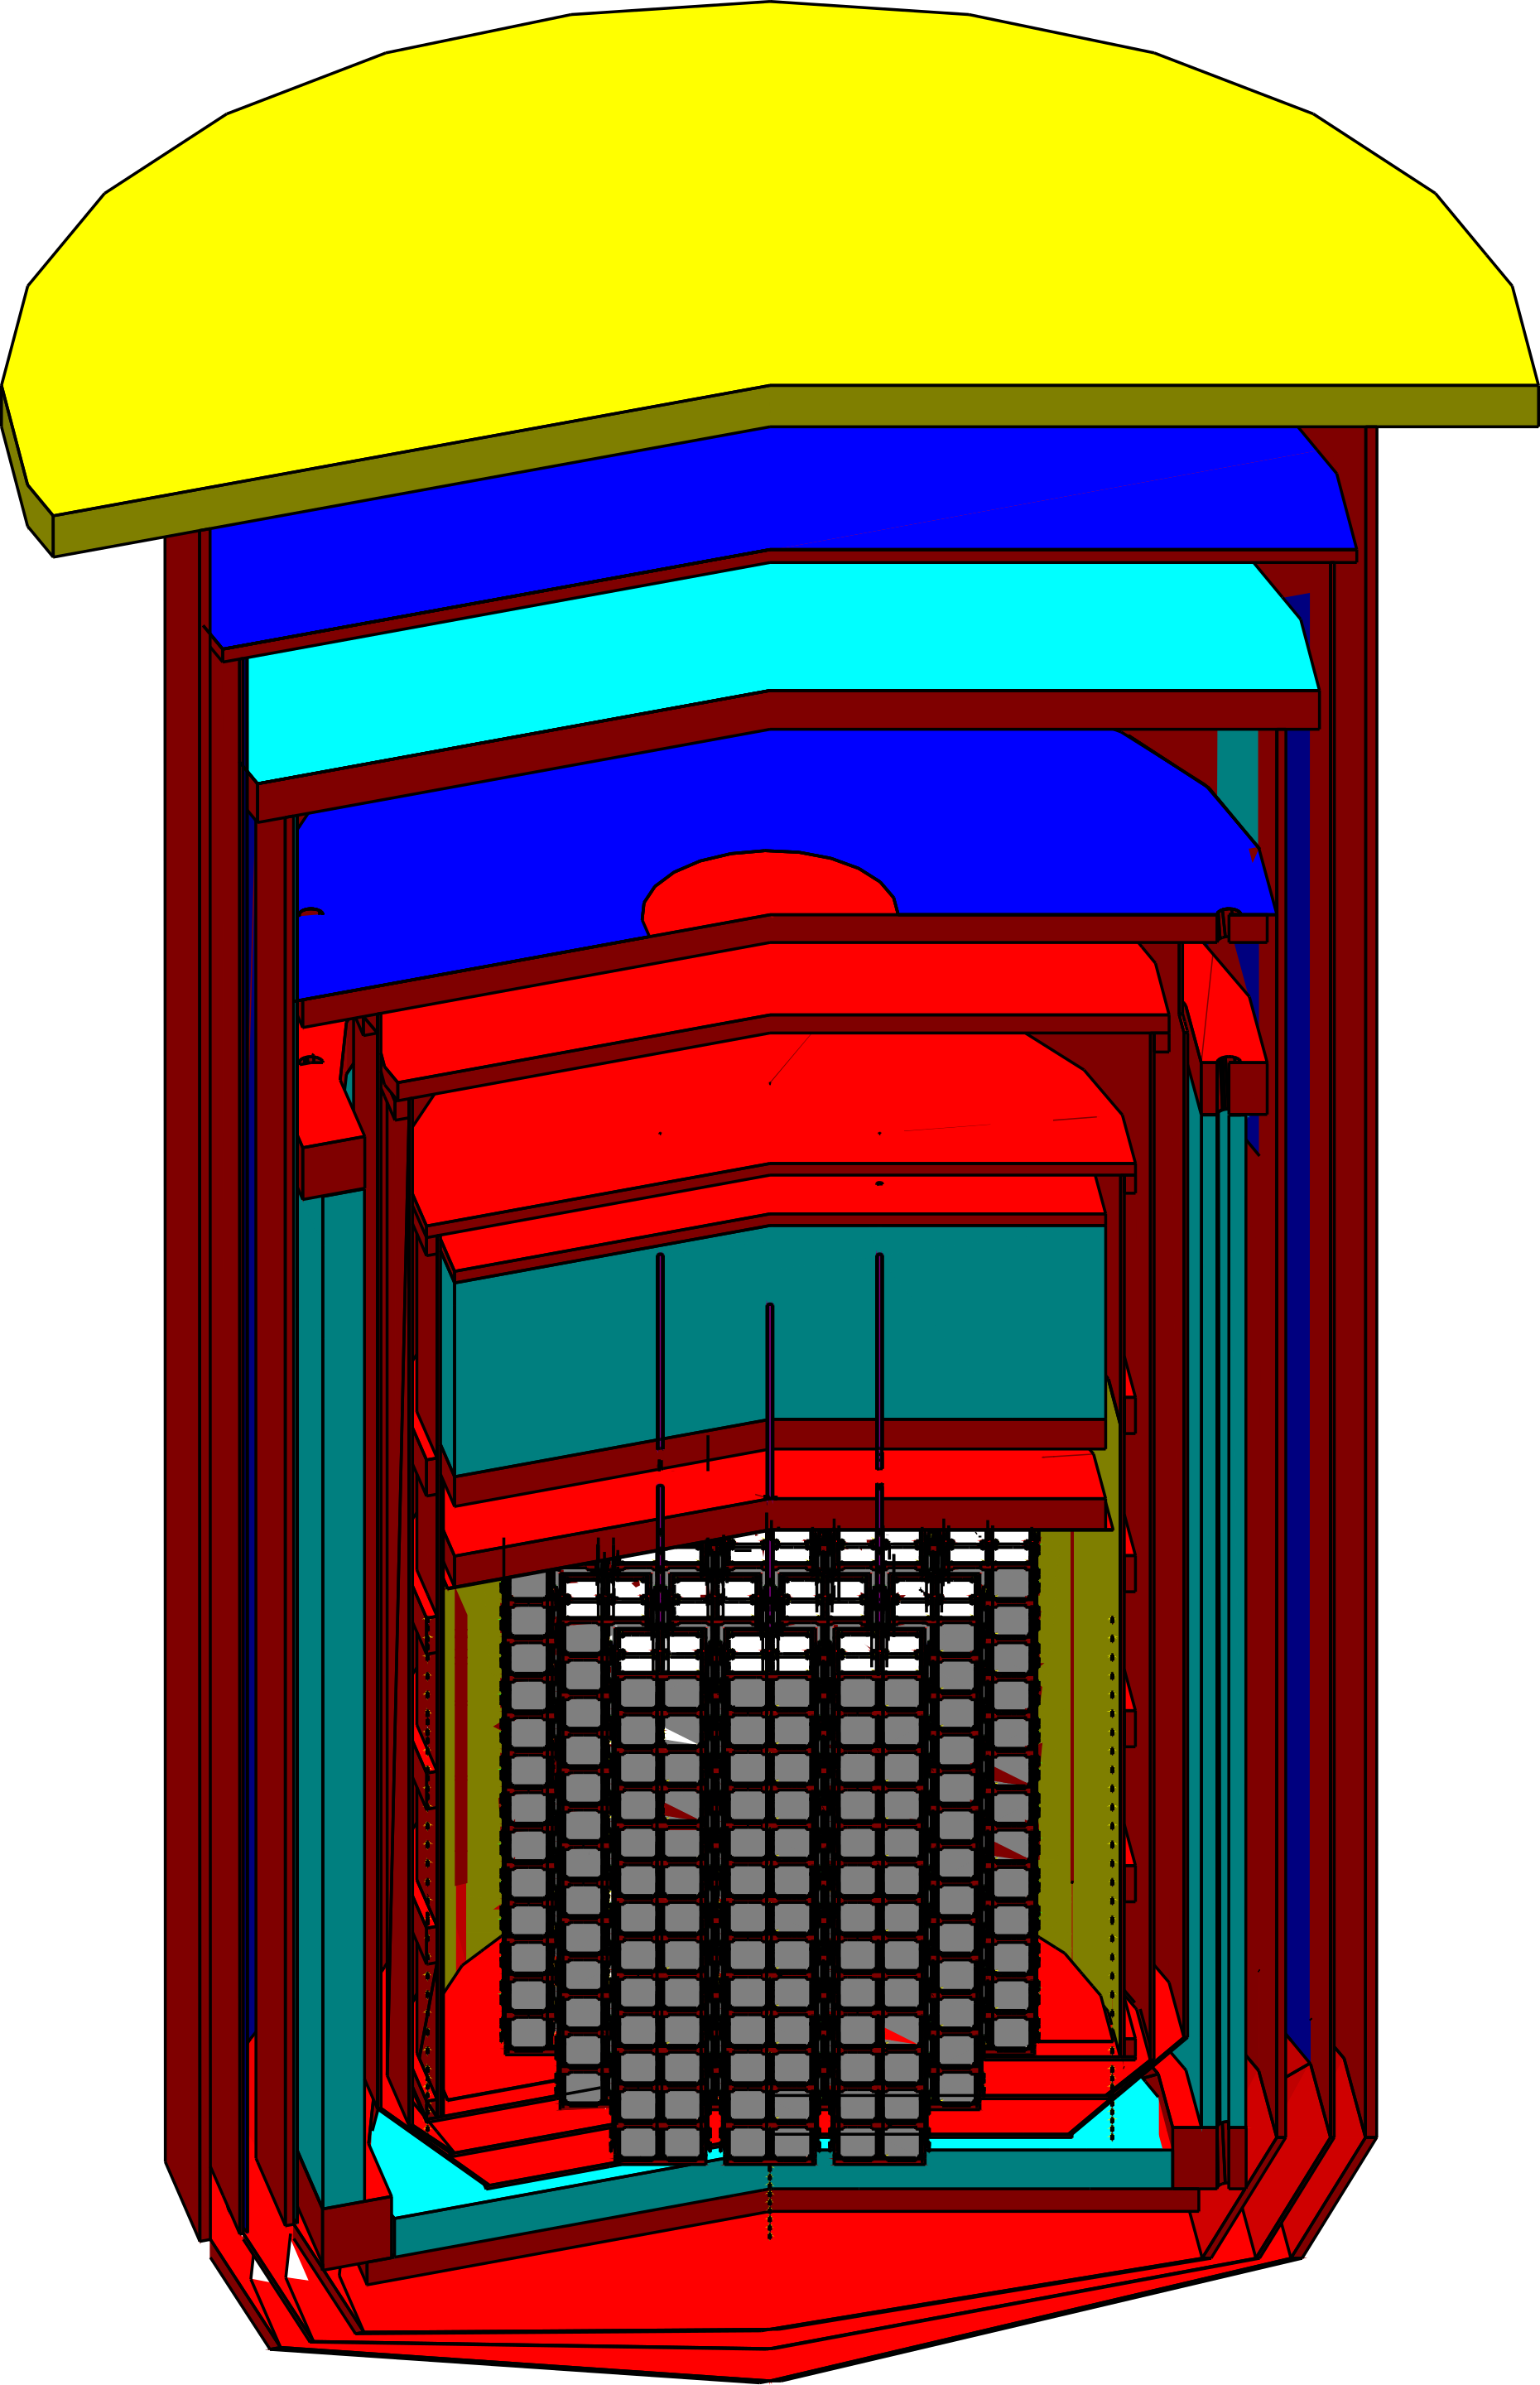
\includegraphics[height=0.6\paperheight]{Figures/CUORE_cryostat_MC.png}
    \caption[A rendering of the CUORE crysotat as it is reconstructed in Geant4.]
    {A rendering of the CUORE cryostat as it is reconstructed in Geant4.
    The shielding is cut away show the inside of the cryostat and some of the tubes for the internal Detector Calibration System.
    \color{red} add labels \color{black}.}
    \label{fig:CUORE_cyrostat_MC}
\end{figure}

\begin{figure}[htbp]
    \centering
    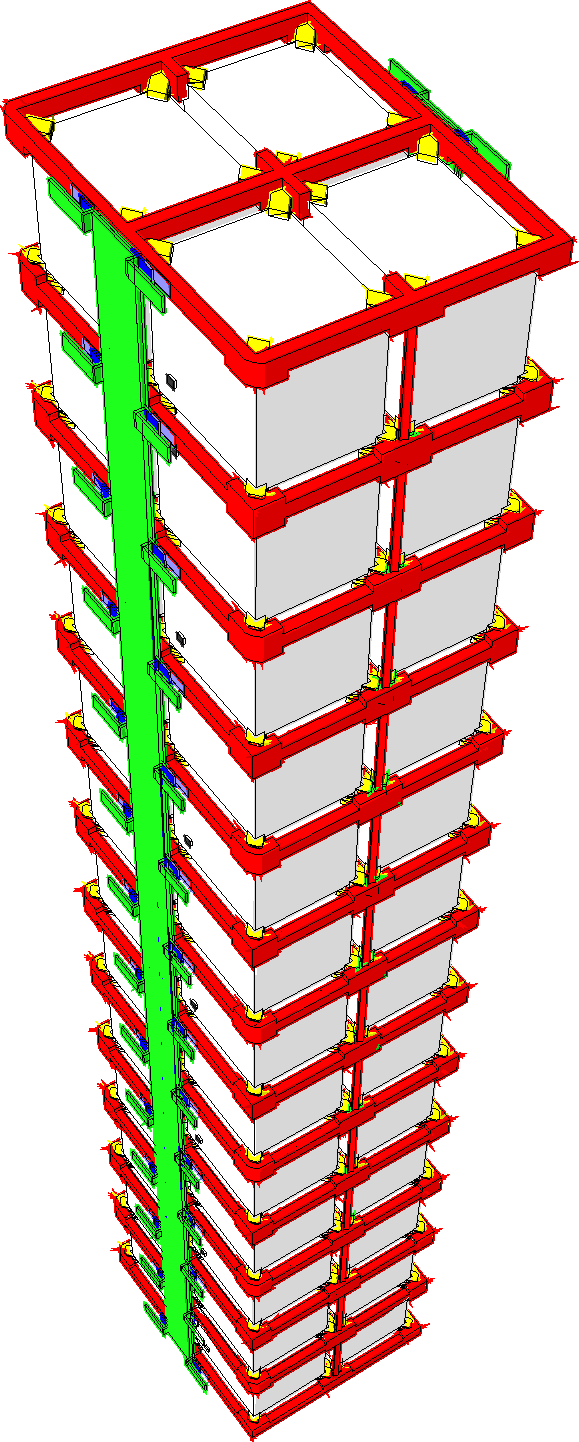
\includegraphics[height=0.4\paperheight]{Figures/Crystals_rotated.pdf}
    \caption[A visualization of the CUORE crystals as they are reconstructed in Geant4.]
    {A visualization of the CUORE crystals as they are reconstructed in Geant4.
    Care is taken to precisely replicate these components in close proximity to the crystals.
    \color{red} add labels \color{black}.}
    \label{fig:CUORE_crystals_MC}
\end{figure}

\section{Simulating Detector Response}
The physics simulation is Geant4 is only one part of the two-step process in performing physics simulations in CUORE.
Geant4 does not take into consideration the actual detector response to the physics, nor does it consider any pileup effects between different primary particles.
To then be able to characterize this response, another software package called \textit{g4cuore} is used.
In this software, the pure physics output from the output of Geant4 is then passed through multiple parameters, including but not limited to
\begin{itemize}
    \item detector resolution
    \item pileup rejection and detector dead time
    \item energy thresholds
    \item coincidences \color{red} maybe same as next? find better wording \color{black}
    \item multi-site events
    \item quenching factors
\end{itemize}

\section{Simulation Benchmarking}

Gotta make sure our simulations are correct!